\let\negmedspace\undefined
\let\negthickspace\undefined
\documentclass[journal]{IEEEtran}
\usepackage[a5paper, margin=10mm, onecolumn]{geometry}
\usepackage{lmodern} 
\usepackage{tfrupee} 
\setlength{\headheight}{1cm}
\setlength{\headsep}{0mm}   

\usepackage{gvv-book}
\usepackage{gvv}
\usepackage{cite}
\usepackage{amsmath,amssymb,amsfonts,amsthm}
\usepackage{algorithmic}
\usepackage{graphicx}
\usepackage{textcomp}
\usepackage{xcolor}
\usepackage{txfonts}
\usepackage{listings}
\usepackage{enumitem}
\usepackage{mathtools}
\usepackage{gensymb}
\usepackage{comment}
\usepackage[breaklinks=true]{hyperref}
\usepackage{tkz-euclide} 
\usepackage{listings}                             
\def\inputGnumericTable{}                                 
\usepackage[latin1]{inputenc}                                
\usepackage{color}                                            
\usepackage{array}                                            
\usepackage{longtable}                                       
\usepackage{calc}                                             
\usepackage{multirow}                                         
\usepackage{hhline}                                           
\usepackage{ifthen}                                           
\usepackage{lscape}
\usepackage{xparse}

\bibliographystyle{IEEEtran}

\title{1.6.12}
\author{EE25BTECH11062 - Vivek K Kumar}

\begin{document}
\maketitle

\renewcommand{\thefigure}{\theenumi}
\renewcommand{\thetable}{\theenumi}

\numberwithin{equation}{enumi}
\numberwithin{figure}{enumi} 

\textbf{Question}:\\
Show that point \myvec{-4 \\ 2} lies on the line segment joining the points \textbf{A} \myvec{-4 \\ 6} and \textbf{B} \myvec{-4 \\ -6}.
\\
\textbf{Solution: }
\begin{table}[H]    
  \centering
  

  \caption{Variables Used}
  \label{tab:1.6.12}
\end{table}
The Collinearity matrix is given by\\
\begin{align}
\myvec{
   \vec{B}-\vec{A} & \vec{C}-\vec{A}
 }^T = \myvec{
   0 & -12 \\
   0 & -4
   }\\
 \xleftrightarrow[]{R_2 \rightarrow {R_2-\frac{1}{3}R_1}}
 \myvec{
   0 & -12
   \\
   0 & 0
   }
\end{align}
Since the rank of the Collinearity matrix is $1$, the points are collinear
\begin{figure}[H]
   \centering
  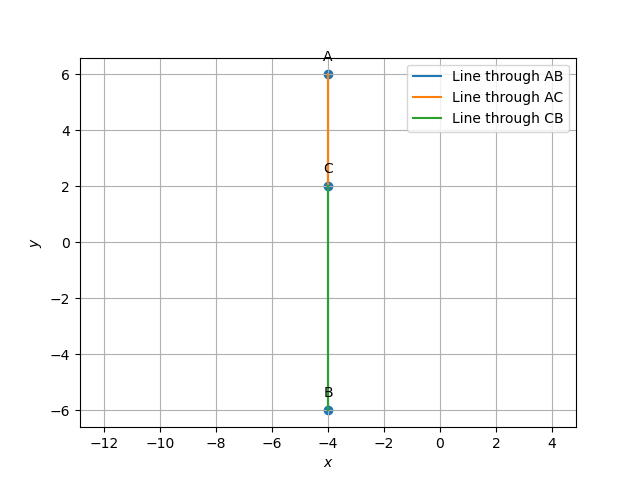
\includegraphics[width=0.64\columnwidth]{figs/fig.png}
   \caption{Line through the given points}
   \label{stemplot}
\end{figure}
\end{document}  

